\runningheader{Oppgave n), frivillig}{}{Side \thepage\ av \numpages}

% ********************************************************
% oppgave n) 
% ********************************************************  
\item[n)]
  Implementer en modell som bruker eksponentialfunksjonen 
   \begin{equation}
     e^{x} 
   \end{equation}
   Ta utgangspunkt i følgende struktur hvor konstantblokken med verdi
   2 innebærer at  $x=2$.

     \begin{figure}[H]
    \centering
    \hspace*{0mm}\scalebox{0.8}{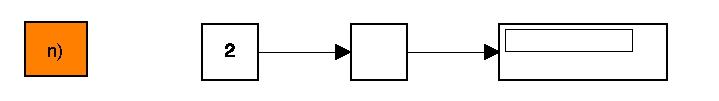
\includegraphics{2n.pdf}}
  \end{figure}
   Bruk igjen 
   en {\sf  Math  Function}-blokk (velg riktig funksjon i menyen)
   og en {\sf    Display}-blokk.

{\color{red}La simuleringstiden fortsatt være  25 sekund.}
Ta med skjermdump av modellen og resultatet.

   
